\documentclass[UTF-8]{article}
\usepackage{amsmath}
\usepackage{graphicx}
\usepackage{float}
\usepackage{subfigure}
\usepackage{amssymb}
\usepackage{esvect}
\usepackage{animate}
\usepackage{framed}
\usepackage{subfigure}
\usepackage[colorlinks]{hyperref}

\setlength{\parindent}{0pt}
\begin{document}
\tableofcontents
\author{ZiLong 201818000807036}
\title{Notes On Ising Model}
\maketitle
\section{Abstract}
The Ising Model, developed by Dr. Ernst Ising, is a mathematical model of ferromagnetism in statistical physics. Dr. Ernst Ising gave the analytical solution in one dimension. The result shows the phase trasition point is at $T=0$. While people believed that here is no phase transition point in two dimensions, the result given by Dr. Onsager showed phase transition point exists indeedly. After that, other methods were developed like mean-field theory, renormalization group and so on. They all indicate two-dimension Ising Model has phase transition. In this article, I will introduce these thoeries and perform some numerical methods such as Metropolis algorithm and cluster algorithm.


\section{Ising Model}
In Ising Model, each atom can adopt two states, corresponding to $S=\{-1,1\}$ where $S$ represents the spin. The spin interaction are dependent of the coupling parameter $J_{ij}$ between the adjacent atoms. For the sake of simplification, I set $J_{ij}=J$, which indicate the system is isotropic. As a result, the Hamiltonian of ferromagnetic Ising Model is:
\begin{equation}
\label{1}
H=-J\sum_{<ij>}S_iS_j,
\end{equation}
where $J>0$ and $S_i\in\{1,-1\}$.\\ \\
The partition function is given by:
\begin{equation}
\label{2}
\mathcal{Z}=\sum_{i}\exp\{-\beta E_i\}=\sum_{S_0}\sum_{S_1}\ldots\sum_{S_N}\exp\{-\beta H\},
\end{equation}
in the canonical ensemble, free energy can be written as:
\begin{equation}
\label{3}
\mathcal{F}=-kTln(\mathcal{Z}).
\end{equation}
At the same time, energy has the form:
\begin{equation}
\label{4}
U=\frac{Tr(exp\{-\beta H\})}{\mathcal{Z}},
\end{equation}
As a result, heat capacity is:
\begin{equation}
C_v=\frac{\partial U}{\partial T}=\frac{\overline{E^2}-\overline{E}^2}{kT^2},
\label{capacity}
\end{equation}
Similarly, magnetic susceptibility can be obtained.
\begin{equation}
\label{mag_sus}
\kappa=\frac{\partial M}{\partial B}=\frac{\overline{M^2}-\overline{M}^2}{kT}.
\end{equation}
As above, Ising Model is described briefly. Next, I will introduce some analytical methods.
\section{Mean Field Theory}
\subsection{Bragg-Williams Approximation}
The main idea of this approximation is to ignore the correlation between the different spins. As a result, the hamiltonian could be simplified:
\begin{equation}
\label{brag_h}
\mathcal{H}=-J\sum_{i}S_i*(\sum_{j}'S_j)=-Jq\overline{S}\sum_{i}S_i,
\end{equation}
where the $\sum_{i}'$ represents sum over the spins near the ith spin. Then, a self-consistent equation could be obtained.
\begin{equation}
\label{cons}
\overline{S}=\frac{\sum_{\{S_i\}}S_1exp\{\beta Jq\overline{S}\sum_{i}S_i\}}{\sum_{\{S_i\}}exp\{\beta Jq\overline{S}\sum_{i}S_i\}}=tanh(\beta Jq\overline{S}).
\end{equation}
It's convenient to get the solution by using iterative method.
\begin{figure}[H]
	\centering
	\includegraphics[width=1\textwidth]{s_bragg.png}
	\caption{solutions for different T}
	\label{fig_1}
\end{figure}
It's easy to make a conclusion that the phase transition point is $\frac{kT}{qJ}=1$, that is, when $q=4,J=1$, $kT_c=4$. The strict solution is about $kT_c=2.269J$, so Bragg-Williams method is a rough approximation.

\subsection{Bethe-Peierls Approximation}
The main idea of this method is to ignore the correlations between three different spins or more. As a result, the hamitonian could be simplified as:
\begin{equation}
\label{bethe_h}
\mathcal{H}_0=-J\sum_{j=1}^{q}S_0S_j-\mu B\sum_{j=1}^{q}S_j,
\end{equation}
where $B$ is the parameter which represents the mean field. Let $\alpha=\frac{\mu B}{kT},\gamma=\frac{J}{kT}$. It's not hard to get the self-consistent equation:
\begin{equation}
\label{bethe_con}
\alpha=\frac{q-1}{2}ln(\frac{cosh(\alpha+\gamma)}{cosh(\alpha-\gamma)}).
\end{equation}
With the same method mentioned in Sec3.1, the average of $S$ is as follows.
\begin{figure}[H]
	\centering
	\includegraphics[width=1\textwidth]{s_bethe.png}
	\caption{solutions for different T}
	\label{fig_2}
\end{figure}
It's also easy to confirm that the phase transition point is about $\frac{kT}{J}=2.88$ for $q=4$. That is, when $J=1$, $kT_c=2.88$, which performs better than Bragg-Williams approximation. 

\section{Metropolis Algorithm}
\subsection{Algorithm Details}
\begin{framed}
1.Locally trail move the current conformation.\\
2.Calculate the energy change caused by the trial move, $dE$.\\
3.If $dE$ is negative, the trial move is allowed; Else allowed the trial move but with a probability $exp(-dE/kT)$. Whether the trial move is allowed or not, a new conformation is thought to be generate.\\
4.Repeat 1,2,3 enough steps.
\end{framed}
\subsection{Results}
\subsubsection{Random Engine}
The first thing of implementing this algorithm is to choose a suitable random engine. With trying a lot of times, I find the random function in random.h which is a library of Cpp is not as good as I imagine. The main reason is that the biggest random number generated is about 60000. Because the random float number is generated by $n$(integer numer generated by random function)/$N$(the biggest number generated by random function), the precision is $1/N$ which is not enough. As a result, I choose a more powerful random engine, which is, mt19937. 
\begin{figure}[H]
	\centering
	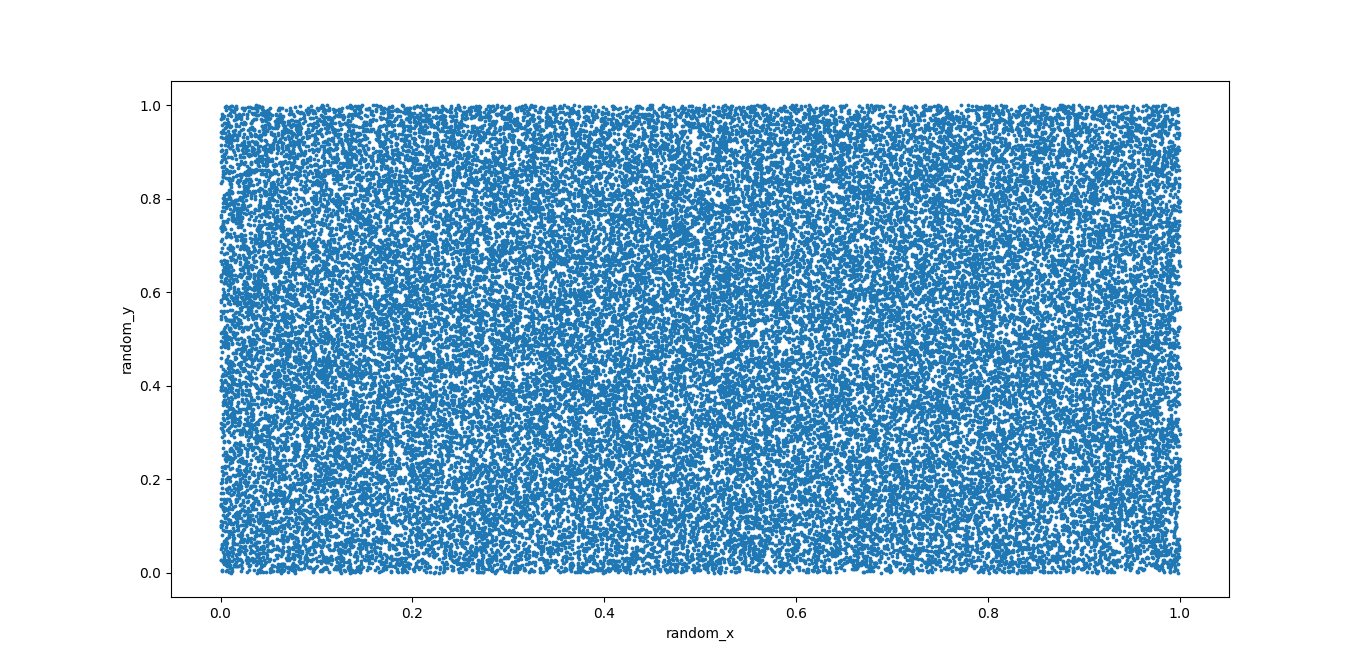
\includegraphics[width=1\textwidth]{random_engine.png}
	\caption{random numbers generated by mt19937}
	\label{fig_3}
\end{figure}
From the Fig.\ref{fig_3}, mt19937 performs well.
\subsubsection{Monte Carlo Cycles}
It would be interesting to investigate how the algorithm behaves with the number of Monte Carlo cycles inceasing.
\begin{figure}[H]
	\centering
	\subfigure[pic1.energy average]{
	\includegraphics[width=5cm]{3.png}
	}
	\subfigure[pic2.energy]{
	\includegraphics[width=5cm]{4.png}	
	}
	\caption{Energy's dynamic change for two different configurations at $kT=3.5$}
\end{figure}
From the figures above, at $kT=3.5$, two different configurations performs well. They both converges quickly, so the chain number could be reduced appropriatly. But things will be different when near the phase transition point, that is, $kT_c=2.269$.
\begin{figure}[H]
	\centering
	\subfigure[pic1.energy average]{
	\includegraphics[width=5cm]{5.png}
	}
	\subfigure[pic2.energy]{
	\includegraphics[width=5cm]{6.png}	
	}
	\caption{Energy's dynamic change for two different configurations at $kT=2.27$}
\end{figure}
As a result, it needs a longer Mente cycles to achieve an equilibrium at $T_c$. So I set $10^6$ cycles when far from $T_c$ and $10^8$ cycles when near $T_c$.\\
\\
Moreover, the accept rate increases with temperature incresing, which indicates that higher temperature means more states the sysytem can have.
\begin{figure}[H]
	\centering
	\includegraphics[width=8cm]{7.png}
	\caption{accept rate versus T}
\end{figure}
Next.

\subsubsection{Numerical Results}
\begin{figure}[H]
	\centering
	\subfigure[pic1.Average Energy at different T]{
	\includegraphics[width=5cm]{8.png}
	}
	\subfigure[pic2.Average Magnet at different T]{
	\includegraphics[width=5cm]{9.png}	
	}
	\caption{Energy and magnet versus kT}
\end{figure}
It's not surprising that the average energy inceaces and average magnet decreses with $kT$ inceasing. When near the $kT_c$, both energy and magnet changes quickly. It's clear that here exists a transition from ferromagnet to paramagnet. Moreover, we could get the $C_v$ and $\kappa$ by using the equation listed in equ.\ref{capacity} and equ.\ref{mag_sus}.\\
\\
From the figures followed, phase transition point exists indeedly. $C_v$ and $\kappa$ increase suddenly, we can even imagine that with $N\rightarrow \infty$, $C_v\rightarrow\infty$ and  $\kappa \rightarrow \infty$ at $T_c$.
\begin{figure}[H]
	\centering
	\subfigure[pic1.$\kappa$ versus T]{
	\includegraphics[width=5cm]{10.png}
	}
	\subfigure[pic2.$C_v$ versus T]{
	\includegraphics[width=5cm]{11.png}	
	}
	\caption{$\kappa$ and $C_V$}
\end{figure}
Next.

\section{Cluster Algorithm--Wolff or Single-Cluster Algorithm}
\subsection{Algorithm Details}
\begin{framed}
1.A spin $i$ is selected at random.\\
2.All nearest neighbors $j$ of this spin are added to the cluster with a probability $p_{ij}=1-exp(-2\beta J)$, provided spins $i$ annd $j$ are parallel and the bond between $i$ and $j$ has not been considered before.\\
3.Each spin $j$ that is indeed added to the cluster is also placed on the stack. Once all neighbors of $i$ have been considered for inclusion in the cluster, a spin is  retrieved from the stack and all its neighbors are considered in turn for inclusion in the cluster as well, following step 2.\\
4.Steps 2 and 3 are repeated iteratively until the stack is empty.\\
5.Once the cluster has been completed, all spins that belong to the cluster are inverted.\\
The implementation can be simplified by a small trick: in step 2,each spin $j$ that is added to the cluster can immediately be inverted. This guranteed that a spin is never added twice. 
\end{framed}
\subsection{Advantages and Disadvantages}
When the model is ferromagnetic ising model, cluster algorithm behaves better, that is, when near the $T_c$, it converges quicker and more accurate. For example, it takes about 10 seconds to get a more accurate results by using cluster method while normal method takes about 100 seconds. The disadvantages are also obvious, this algorithm is designed for a more special model. When a magnetic field is applied, it does not work.

\subsection{Results}
\begin{figure}[H]
	\centering
	\subfigure[pic1.energy distribution at T=1.5k]{
	\includegraphics[width=5.5cm]{16.png}
	}
	\subfigure[pic2.energy distribution at T=3.5k]{
	\includegraphics[width=5.5cm]{17.png}	
	}
	\caption{Energy distribution}
\end{figure}
It has a wider distribution at $kT=3.5$ which is reasonable. Next, I will show why cluster algorithm behaves better.
\begin{figure}[H]
	\centering
	\subfigure[pic1.initial state]{
	\includegraphics[width=5.5cm]{18.jpg}
	}
	\subfigure[pic2.state after 100 steps]{
	\includegraphics[width=5.5cm]{19.jpg}	
	}
	\caption{State evolution at kT=1.5}
\end{figure}
At a low temperature, state evolves at a breathtaking pace. It takes a fewer time to come to equilibrium.
\begin{figure}[H]
	\centering
	\subfigure[pic1.E]{
	\includegraphics[width=5cm]{12.png}
	}
	\subfigure[pic2.H]{
	\includegraphics[width=5cm]{14.png}	
	}
	\caption{H and E}
\end{figure}
\begin{figure}[H]
	\centering
	\subfigure[pic1.$C_v$]{
	\includegraphics[width=5.5cm]{13.png}
	}
	\subfigure[pic2.$\kappa$]{
	\includegraphics[width=5.5cm]{15.png}	
	}
	\caption{$\kappa$ and $C_v$}
\end{figure}
From the figures above, the error is smaller than metropolis algorithm. Finally, I want to get the $T_c$ from the simulated data. That's not difficult. when $T\rightarrow (T_c-0)$, $M=\alpha(\frac{T_c-T}{T})^\beta$, so I just use this formula to fit the data.
\begin{figure}[H]
	\centering
	\includegraphics[width=9cm]{20.png}
	\caption{Phase transition point}
\end{figure}
The fitting result is $kT_c=2.22$, which is close to the right answer $kT_c=2.269$.
\section{Conclusion}
I introduce some theories about ising model briefly, then I spend much more time on the simulation method  especilly metropolis algorithm and cluster algorithm. Procedural details will not be presented here. More information is available on my GitHub https://github.com/ZiLongLiqb/Isingmodel2d.
\begin{thebibliography}{1}
\bibitem{cluster} E.Luijten. Introduction to Cluster Monte Carlo Algorithm, Lect. Notes Phys. 703,13-38(2006)
\end{thebibliography}
\end{document}